\chapter{SYSTEM DEVELOPMENT}\label{SYSTEM DEVELOPMENT}
This chapter discusses the process of the development of the whole system. There were two approaches to this research. One approach included classical machine learning algorithms to predict the classes of cervical cells. Another approach was CNN-based federated learning technique in order to achieve the same objectives.
\section{Data Collection}

The dataset used for the development of classic ML and base model of FL architecture has been taken from Kaggle namely SipakMed Database \cite{ar29}, which is the largest dataset available. The database contains images of isolated cells, taken manually from the cluster cell images of Pap smear slides. The dataset contains a total of 4049 images, each of size 66X66. The cell images are divided into five categories in which there are 813 images of Dyskeratotic cells, 825 images of Koilocytotic cells, 793 images of Metaplastic cells, 787 images of Parabasal cells, and lastly 831 images of Superficial-Intermediate cells.

\begin{figure}[H]
\centering
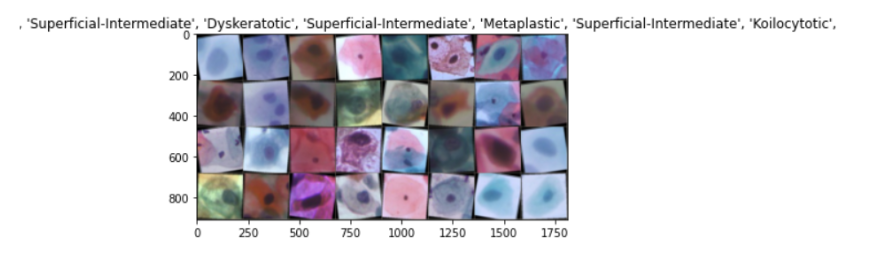
\includegraphics[width=170mm,height=55mm]{figures/data_visualization.png}
\caption{Visualization of the SIPAKMED dataset}
\label{Visualization of the SIPAKMED dataset}
\end{figure}

\section{Developing the Classical ML models}
\subsection{Data Pre-processing} \

\textbf{a. Gray-scale Conversion: }
Gray-scale conversion of images facilitates the simplification of algorithms and also removes the difficulties associated with computational requirements. Grayscale compression reduces an image to its most basic pixel.\

\textbf{b. Flattening: }
In order to feed information from a 1-D array into a classification model, a technique known as flattening is utilized to transform multidimensional arrays into 1-D arrays.The multidimensional image array was flattened before processing the data to the ml models because 1-D arrays use less memory and  multi-dimensional arrays require more memory. Flattening aids in minimizing memory usage as well as speeding up model training.\

\textbf{c. Resizing the images: }
We resized the images to the size of 28x28 pixels and created a dataframe of 784 pixels for each images. \

\textbf{d. Rescaling the images: }
Each image was re-scaled from pixel range to the range of 0 to 255. \

\textbf{e. Train-Test Splitting: }
The dataset was divided into train and test images with a test ratio of 20\%. \

\textbf{f. Handling Imbalanced Data: }
After train-test splitting, Synthetic Minority Oversampling Technique, or SMOTE was used for handling imbalanced data. Figure 5.2 shows the effect of the process. Before the 5 cells were found to have variations in total numbers of data, but after the application of SMOTE the amount of data in each class gets equally distributed, and thus aiding in removing the imbalance of data. 

\begin{figure}[H]
\centering
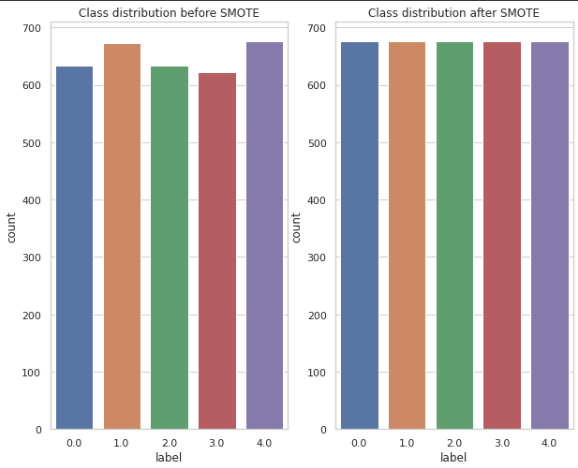
\includegraphics[width=100mm,height=50mm]{figures/smote.png}
\caption{Class distribution before and after applying SMOTE}
\label{DLAccuracy}
\end{figure}

\subsection{Result Analysis of the ML Models}
A confusion matrix is the table used to describe the performance of a classification model or classifier on a set of test data for which the true values are known. A confusion matrix is used to measure the performance of a classifier in depth. Figure-5.3 shows the confusion matrices for train data and Figure-5.4 shows the confusion matrices for test data. Here the top 5 models are as follows: LightGBM, HGB+LightGBM, HGB, Extratrees and SVM. The lightgbm model is found to perform better than the other models.

\begin{figure}[H]
    \centering
    \begin{subfigure}{.55\textwidth}
        \centering
        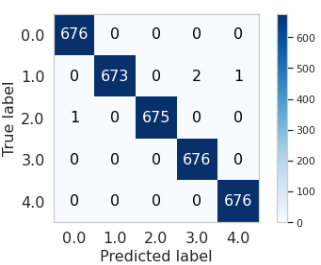
\includegraphics[width=.55\linewidth]{figures/lgbm_train.png}
        \caption{}
        \label{fig:sub1}
    \end{subfigure}%
    \begin{subfigure}{.55\textwidth}
        \setcounter{subfigure}{1} % set next caption to b
        \centering
        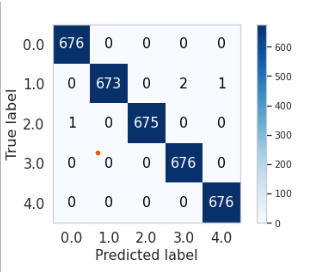
\includegraphics[width=.55\linewidth]{figures/lgbm_hgb_train.png}
        \caption{}
        \label{fig:sub2}
    \end{subfigure}\\
    \begin{subfigure}{.55\textwidth}
        \setcounter{subfigure}{2} % set next caption to c
        \centering
        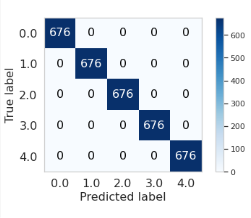
\includegraphics[width=.55\linewidth]{figures/hgb_train.png}
        \caption{}
        \label{fig:sub3}
    \end{subfigure}%
    \begin{subfigure}{.55\textwidth}
        \setcounter{subfigure}{3} % set next caption to d
        \centering
        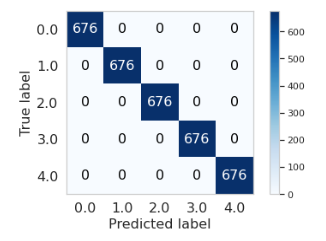
\includegraphics[width=.55\linewidth]{figures/xtratrees_train.png}
        \caption{}
        \label{fig:sub4}
    \end{subfigure}   
\end{figure}
\begin{figure}[H]
    \centering
    \ContinuedFloat
     
    \bigskip
    \begin{subfigure}{.55\textwidth}
        \setcounter{subfigure}{4} % set next caption to c
        \centering
        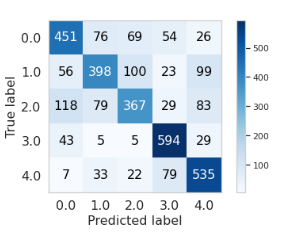
\includegraphics[width=.55\linewidth]{figures/svm_train.png}
        \caption{}
        \label{fig:sub3}
    \end{subfigure}%
    
    \caption{Confusion Matrix of true train vs predicted train for (a) LightGBM, (b) HGB + LightGBM, (c) HGB, (d) Extratrees and (e) SVM}\label{fig:main}
\end{figure}

\begin{figure}[H]
    \centering
     \begin{subfigure}{.55\textwidth}
        \centering
        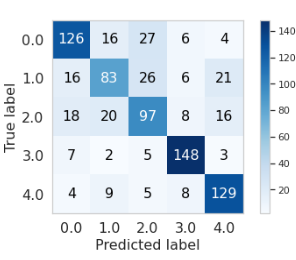
\includegraphics[width=.55\linewidth]{figures/lgbm_test.png}
        \caption{}
        \label{fig:sub1}
    \end{subfigure}%
    \begin{subfigure}{.55\textwidth}
        \setcounter{subfigure}{1} % set next caption to b
        \centering
        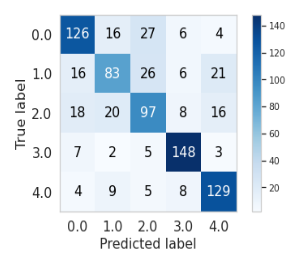
\includegraphics[width=.55\linewidth]{figures/lgbm_hgb_test.png}
        \caption{}
        \label{fig:sub2}
    \end{subfigure}\\
    \bigskip
    \begin{subfigure}{.55\textwidth}
        \setcounter{subfigure}{2} % set next caption to c
        \centering
        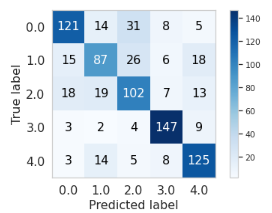
\includegraphics[width=.55\linewidth]{figures/hgb_test.png}
        \caption{}
        \label{fig:sub3}
    \end{subfigure}%
    \begin{subfigure}{.55\textwidth}
        \setcounter{subfigure}{3} % set next caption to d
        \centering
        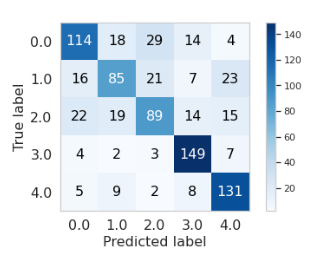
\includegraphics[width=.55\linewidth]{figures/xtratrees_test.png}
        \caption{}
        \label{fig:sub4}
    \end{subfigure}  
    \begin{subfigure}{.55\textwidth}
        \setcounter{subfigure}{4} % set next caption to c
        \centering
        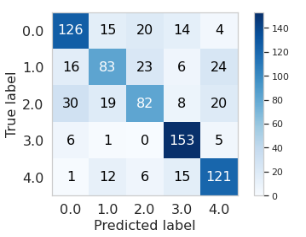
\includegraphics[width=.55\linewidth]{figures/svm_test.png}
        \caption{}
        \label{fig:sub3}
    \end{subfigure}%
     \caption{Confusion Matrix of true test vs predicted test for (a) LightGBM, (b) HGB + LightGBM, (c) HGB, (d) Extratrees and (e) SVM}\label{fig:main}
\end{figure}






\subsubsection{Evaluation Metrics}
Table-5.1 shows the evaluation matrics of train data, where the LightGBM and HGB+LightGBM are found to provide same accuracy. Similarly, HGB, Xtra Trees and KNN, Decision trees are also found to perform similar. In the table-5.2 the evaluation metrics of the test data are sorted according to the test accuracy. 


\begin{table}[htb]
\caption{Evaluation Metrics of Train Data}
\centering
    \scalebox{0.9}{
    \begin{tabular}{|l|l|l|l|l|}
    \hline
        Model &  Accuracy  & Precision  & Recall  & F1\_score   \\ \hline
        LightGBM  & 0.999  &  0.999  &  0.999  &  0.999   \\ \hline
        HGB+LGBM & 0.999  & 0.999  & 0.999  & 0.999   \\ \hline
        HGB & 1  & 1  & 1  & 1   \\ \hline
        Xtra Trees  & 1  & 1  & 1  & 1   \\ \hline
        SVM  & 0.694  & 0.69  & 0.694  & 0.689  \\ \hline
        SVM\_Grid\_Search  &  0.872  &  0.875  &  0.872  &  0.872  \\ \hline
        Gradient Boosting  & 0.846  & 0.847  & 0.846  & 0.845  \\ \hline
        XGBOOST  & 0.77  & 0.775  & 0.77  & 0.768  \\ \hline
        MLP  & 0.705  & 0.716  & 0.705  & 0.704 \\ \hline
        HGB + XGBoost  & 0.768  & 0.771  & 0.768  & 0.766  
        \\ \hline
        KNN  &  1  &  1  &  1  &  1   \\ \hline
        Decision Tree  & 1  & 1  & 1  & 1 \\ \hline
        AdaBoost  & 0.481  & 0.496  & 0.481  & 0.483  \\ \hline
        Random Forest  & 0.477  & 0.488  & 0.477  & 0.449   \\ \hline
        Gaussian Naive Bayes  & 0.408  & 0.449  & 0.408  & 0.361  \\ \hline
    \end{tabular}
    }
\end{table}

\begin{table}[!ht]
\caption{Evaluation Metrics of Test Data}
\centering
\scalebox{0.9}{
    \begin{tabular}{|l|l|l|l|l|}
    \hline
 Model &  Accuracy  & Precision  & Recall  & F1\_score \\ \hline
        LightGBM  &  0.72  &  0.714  &  0.718  &  0.714 \\ \hline
        HGB+LGBM & 0.72  & 0.714  & 0.718  & 0.714   \\ \hline
        HGB & 0.719  & 0.715  & 0.717  & 0.715   \\ \hline
        Xtra Trees  & 0.701  & 0.694  & 0.701  & 0.694  \\ \hline
        SVM  & 0.698  & 0.689  & 0.695  & 0.688   \\ \hline
        SVM\_Grid\_Search  &  0.695  &  0.685  &  0.692  &  0.687   \\ \hline
        Gradient Boosting  & 0.686  & 0.678  & 0.685  & 0.678   \\ \hline
        XGBOOST  & 0.683  & 0.678  & 0.681  & 0.674  \\ \hline
        MLP  & 0.673  & 0.681  & 0.67  & 0.668  \\ \hline
        HGB + XGBoost  & 0.669  & 0.662  & 0.667  & 0.66  \\ \hline
        KNN  &  0.562  &  0.567  &  0.555  &  0.539  \\ \hline
        Decision Tree  & 0.535  & 0.527  & 0.531  & 0.529   \\ \hline
        AdaBoost  & 0.485  & 0.503  & 0.482  & 0.486   \\ \hline
        Random Forest  & 0.456  & 0.46  & 0.448  & 0.424   \\ \hline
        Gaussian Naive Bayes  & 0.435  & 0.456  & 0.423  & 0.369  \\ \hline
    \end{tabular}
    }
    \label{table: Evaluation Metrics of Test Data}
\end{table}

\pagebreak

\subsubsection{Cross Validation Results} 
Cross Validation evaluates the model using different chunks of the data set as the validation set. In K-fold cross validation, ‘K’ represents the number of groups that a given dataset is to be split into. The dataset is divided into k parts, and  in different iterations, one part is used for testing the model, while the other remaining parts are used for training purposes. Then after k-iterations, an average of all the individual scores is done to obtain the final score. In this study, 5-fold cross validation is applied on the entire dataset. 

In table 5.3, 5-fold cross validation results are shown for training set and in table 5.4, 5-fold cross validation results are shown for validation set. Here the top 6 models which performs best on training data are: Histogram Gradient Boosting (HGB) + LightGBM, LightGBM, Histogram Gradient Boosting, Extreme Gradient Boosting (XGBoost), Histogram Gradient Boosting + Extreme Gradient Boosting and Extra trees. 

\begin{table}[!ht]
    \centering
    \caption{Cross Validation Results for Training Set}
    \begin{tabular}{|l|l|l|l|l|}
    \hline
        Model\_name & \makecell{Mean\\ Training\\ Accuracy\\ (in percentage)} & \makecell{Mean\\ Training\\ Precision} & \makecell{Mean\\ Training\\ Recall} & \makecell{Mean\\ Training\\ F1 Score} \\ \hline
        HGB + LightGBM & 100 & 1 & 1 & 1 \\ \hline
        LightGBM & 100 & 1 & 1 & 1 \\ \hline
        HGB & 100 & 1 & 1 & 1 \\ \hline
        XGBoost & 100 & 1 & 1 & 1 \\ \hline
        HGB + XGBoost & 100 & 1 & 1 & 1 \\ \hline
        Extra Trees & 100 & 1 & 1 & 1 \\ \hline
        Gradient Boosting & 84.90985253 & 0.849366961 & 0.849433242 & 0.848145364 \\ \hline
        SVM\_Grid\_Search & 86.81156926 & 0.870367728 & 0.868133276 & 0.86773494 \\ \hline
        SVM & 69.93081236 & 0.696427677 & 0.699306189 & 0.693327781 \\ \hline
        MLP & 68.77627221 & 0.696460777 & 0.688059482 & 0.683649547 \\ \hline
        KNN & 100 & 1 & 1 & 1 \\ \hline
        Decision Tree & 100 & 1 & 1 & 1 \\ \hline
        Random Forest & 47.24004132 & 0.478736029 & 0.47345261 & 0.447405383 \\ \hline
        Adaboost & 47.97471785 & 0.496924946 & 0.480725118 & 0.483934274 \\ \hline
        Naive Bayes & 41.37440111 & 0.448321855 & 0.412054824 & 0.363859397 \\ \hline
    \end{tabular}
\end{table}

\begin{table}[!ht]
    \centering
    \caption{Cross Validation Results for Validation Set}
    \begin{tabular}{|l|l|l|l|l|}
    \hline
         Model\_name & \makecell{Mean\\ Validation\\ Accuracy\\ (in percentage)} & \makecell{Mean\\ Validation\\ Precision} & \makecell{Mean\\ Validation\\ Recall} & \makecell{Mean\\ Validation\\ F1 Score} \\ \hline
        HGB + LightGBM & 70.56133925 & 0.701983809 & 0.706121962 & 0.702796063 \\ \hline
        LightGBM & 70.56133925 & 0.701983809 & 0.706121962 & 0.702796063 \\ \hline
        HGB & 69.72107006 & 0.693044681 & 0.697875695 & 0.694534567 \\ \hline
        XGBoost & 69.3016527 & 0.688479078 & 0.693655077 & 0.689358876 \\ \hline
        HGB + XGBoost & 69.05428131 & 0.685542518 & 0.691234928 & 0.686148781 \\ \hline
        Extra Trees & 68.9553938 & 0.684843567 & 0.690223384 & 0.684319871 \\ \hline
        Gradient Boosting & 66.56002686 & 0.661458162 & 0.6663828 & 0.661037635 \\ \hline
        SVM\_Grid\_Search & 66.21407316 & 0.657991898 & 0.66290078 & 0.65762497 \\ \hline
        SVM & 63.79355705 & 0.631791996 & 0.638140273 & 0.629743308 \\ \hline
        MLP & 60.87915274 & 0.610446237 & 0.609444673 & 0.600964649 \\ \hline
        KNN & 53.02635474 & 0.553604967 & 0.533233073 & 0.515285127 \\ \hline
        Decision Tree & 51.0741809 & 0.508561817 & 0.511054756 & 0.508912903 \\ \hline
        Random Forest & 46.40647652 & 0.46922437 & 0.465063736 & 0.439952827 \\ \hline
        Adaboost & 44.06079751 & 0.457688023 & 0.441604779 & 0.444543543 \\ \hline
        Gaussian Naive Bayes & 41.17035206 & 0.444675024 & 0.409996198 & 0.360853211 \\ \hline
    \end{tabular}
\end{table}

% \begin{figure}[H]
% \centering
% 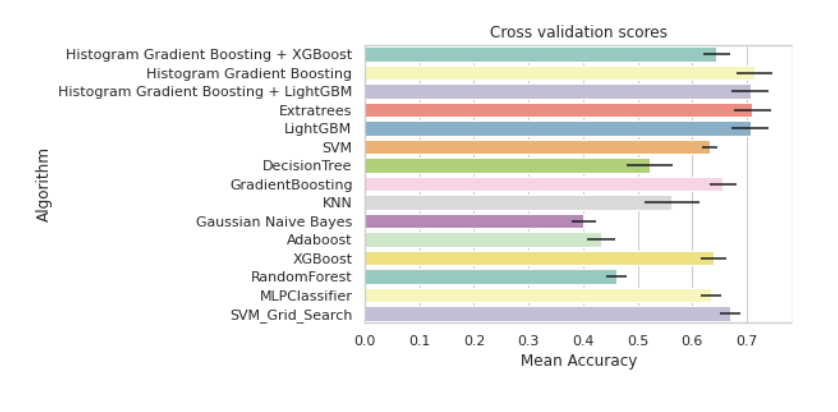
\includegraphics[width=160mm,height=80mm]{figures/cvresult.png}
% \caption{10 Fold cross-validation results}
% \label{DLAccuracy}
% \end{figure}

\pagebreak

\section{Development of Federated Learning Architecture}
\subsection{Data Partitioning}
For developing a system similar to horizontal data-partitioning system, the SIPAKMED dataset was divided into three training sets for three clients, each having 28\% images of the whole dataset and a single test set which is 15\% of the whole dataset. Table 5.5 shows how many training images of each classes a single client got after dividing the whole dataset.    
\begin{table}[!ht]
\centering
    \caption{Division of images on 3 clients}
    \begin{tabular}{|l|l|l|l|l|}
    \hline
         Class No. & Client\_1(28\%)  & Client\_2(28\%) & Client\_3(28\%)  & Test (15\%) \\ 
         \hline
         Class1 & 230  & 230  &  230  &  123 \\ 
         \hline
         Class2 & 230  & 230  & 228  & 137   \\ 
         \hline
         Class3 & 215  & 215  & 215  & 148   \\ 
         \hline
         Class4 & 215  & 215  & 215  & 142   \\ 
         \hline
         Class5 & 230  & 235  & 231  & 135  \\ 
         \hline
    \end{tabular}
\end{table}

\subsection{Data Augmentation}
% train_datagen = tf.keras.preprocessing.image.ImageDataGenerator(zoom_range = 0.2, shear_range = 0.2 , rescale = 1./255 , horizontal_flip=True)
The Keras ImageDataGenerator class was used for numerous augmentation methods, including zooming, shearing, rescaling and horizontal flips.

\subsection{Development of the Foundation Model}

Keras model for cervical cell classification was developed using a Convolutional Neural Networks.

\subsubsection{Input Shape}
The input\_shape argument for the 2 CNN Model was set to (66, 66, 3). This specifies the shape of the input images that the model had been trained on. The input images were expected to have a width of 66 pixels, a height of 66 pixels, and 3 color channels (corresponding to the Red, Green, and Blue color channels).


\subsubsection{Output Shape} 
The final output shape of the Keras model was 5 as in the number of cell classes. These five values were output by the last layer of the model, which has a sigmoid activation function. 

\subsubsection{Development of the CNN architecture} 

Description for the two CNN architectures developed as a foundation model for the FL architecture are given below:

\subsubsection{Layers utilized in the CNN architecture 1}
\begin{itemize}
    \item \textit{Conv2D(filters=16, kernel_size= (3,3), activation= 'relu', input_shape=(66,66,3)):} This is a convolutional layer with 16 filters of size (3, 3) and a ReLU activation function.
    \item \textit{Conv2D(filters=32, kernel_size=(3,3), activation='relu'):} This is a convolutional layer with 32 filters of size (3, 3) and a ReLU activation function.
    \item \textit{MaxPooling2D((2, 2)):}This is a max pooling layer that reduces the spatial dimensions of the output of the previous layer by a factor of 2. The layer takes the maximum value in each 2x2 window of the input.
    \item \textit{Conv2D(filters=64, kernel_size=(3,3), activation='relu'):} This is another convolutional layer with 64 filters of size (3, 3) and a ReLU activation function.
    \item \textit{MaxPooling2D((2, 2)):}This is a max pooling layer that reduces the spatial dimensions of the output of the previous layer by a factor of 2. The layer takes the maximum value in each 2x2 window of the input.
    \item \textit{Conv2D(filters=128, kernel_size=(3,3), activation='relu'):} This is another convolutional layer with 128 filters of size (3, 3) and a ReLU activation function.
    \item \textit{MaxPooling2D((2, 2)):}  This is another max pooling layer that reduces the spatial dimensions of the output of the previous layer by a factor of 2.
    \item \textit{Dropout(rate=0.25)}  This is a dropout layer as a regularization technique for overfitting problem.
    \item \textit{Flatten():} This layer flattens the output of the previous layer into a 1D tensor, which can then be passed to a fully connected layer.
    \item \textit{Dense(64, activation='relu'):}  This is a fully connected layer with 64 units and a ReLU activation function.
    \item \textit{Dropout(rate=0.25)}  This is a dropout layer as a regularization technique for overfitting problem.
    \item \textit{Dense(5, activation='sigmoid'):} This is the final output layer with 5 units (one for each class) and a sigmoid activation function. The linear activation function means that the output of the layer is not constrained to a particular range, so it can take any real value.
    
\end{itemize}

\begin{table}[!ht]
\centering
    \caption{CNN architecture 1}
    \begin{tabular}{|l|l|l|l|}
    \hline
        Name & Type & Shape & Parameters \\ \hline
        conv2d\_44 & Conv2D & (None, 64, 64, 16) & 448 \\ \hline
        conv2d\_45 & Conv2D & (None, 62, 62, 32) & 4640 \\ \hline
        max\_pooling2d\_33 & MaxPooling2D & (None, 31, 31, 32) & 0 \\ \hline
        conv2d\_46 & Conv2D & (None, 29, 29, 64) & 18496 \\ \hline
        max\_pooling2d\_34 & MaxPooling2D & (None, 14, 14, 64) & 0 \\ \hline
        conv2d\_47 & Conv2D & (None, 12, 12, 128) & 73856 \\ \hline
        max\_pooling2d\_35 & MaxPooling2D & (None, 6, 6, 128) & 0 \\ \hline
        dropout\_22 & Dropout & (None, 6, 6, 128) & 0 \\ \hline
        flatten\_11 & Flatten & (None, 4608) & 0 \\ \hline
        dense\_33 & Dense & (None, 64) & 294976 \\ \hline
        dropout\_23 & Dropout & (None, 64) & 0 \\ \hline
        dense\_34 & Dense & (None, 5) & 325 \\ \hline
        Total params: 392,741 & ~ & ~ & ~ \\ \hline
        Trainable params: 392,741 & ~ & ~ & ~ \\ \hline
        Non-trainable params: 0 & ~ & ~ & ~\\ \hline
    \end{tabular}
\end{table}

% hyperparameters table
\begin{table}[!ht]
\caption{Hyperparameter set 1 used for CNN Model 1}
\centering
\begin{tabular}{p{6cm}p{6cm}}
\hline
\small \textbf{Parameters Used} & \small \textbf{Values}  \\
\hline
\small \textbf{Number of Conv2D layers} & \small 4 \\ 

\small \textbf{Number of MaxPooling2D layers} & \small 3  \\

\small \textbf{Number of Dense layers} & \small 2 \\

\small \textbf{Number of Dropouts} & \small 2 \\

\small \textbf{Number of units in the Dense layers} & \small 64, 5 \\

\small \textbf{Activation functions used} & \small ReLU for Conv2D layers and Dense layers, and sigmoid for the output layer \\ 

\small \textbf{Loss function} & \small categorical_crossentropy \\ 

\small \textbf{Optimizer} & \small Adam \\ 

\small \textbf{Input image size} & \small 66 x 66 x 3 (RGB image with 66 height, 66 width, and 3 channels) \\ 

\small \textbf{Batch Size} & \small 100 \\ 

\small \textbf{Total Communication Round} & \small 10 \\

\small \textbf{Steps Per Epoch for Local Train} & \small 3 \\ 

\small \textbf{Number of Epochs for Local Train} & \small 150 \\ 

\small \textbf{Learning Rate} & \small 0.013 \\ 
\hline
\end{tabular}
\label{table:hyperparameters}
\end{table}

\begin{table}[H]
    \caption{Evaluation Metrics for CNN Architecture 1 and Hyper-parameter set 1}
    \centering
    \begin{tabular}{|l|l|l|l|l|l|l|}
    \hline
        Model & Hyper-parameter Set & Test Accuracy & Precision & Recall & f1-score & roc\_auc\_score \\ \hline
        CNN 01 & 1 & 82.18\% & 82.59\% & 83.47\% & 82.62\% & 89\% \\ \hline
    \end{tabular}
\end{table}

To increase the performance of CNN model displayed in Table 5.8, there were changes made in the architecture as well as two different hyper-parameter sets were used. 

\subsubsection{Layers utilized in the CNN architecture 2}
\begin{itemize}
    \item \textit{Conv2D(filters=16, kernel_size= (3,3), activation= 'relu', input_shape=(66,66,3)):} This is a convolutional layer with 16 filters of size (3, 3) and a ReLU activation function.
    \item \textit{Conv2D(filters=32, kernel_size=(3,3), activation='relu'):} This is a convolutional layer with 32 filters of size (3, 3) and a ReLU activation function.
    \item \textit{MaxPooling2D((2, 2)):}This is a max pooling layer that reduces the spatial dimensions of the output of the previous layer by a factor of 2. The layer takes the maximum value in each 2x2 window of the input.
    \item \textit{BatchNormalization():} This layer is used to prevent model overfitting.
    \item \textit{Conv2D(filters=64, kernel_size=(3,3), activation='relu'):} This is another convolutional layer with 64 filters of size (3, 3) and a ReLU activation function.
    \item \textit{MaxPooling2D((2, 2)):}  This is another max pooling layer that reduces the spatial dimensions of the output of the previous layer by a factor of 2.
    \item \textit{Conv2D(filters=128, kernel_size=(3,3), activation='relu'):} This is another convolutional layer with 128 filters of size (3, 3) and a ReLU activation function.
    \item \textit{MaxPooling2D((2, 2)):}  This is another max pooling layer that reduces the spatial dimensions of the output of the previous layer by a factor of 2.
    \item \textit{Dropout(rate=0.25)}  This is a dropout layer as a regularization technique for overfitting problem.
    \item \textit{Flatten():} This layer flattens the output of the previous layer into a 1D tensor, which can then be passed to a fully connected layer.
    \item \textit{Dense(256, activation='relu'):}  This is a fully connected layer with 256 units and a ReLU activation function.
    \item \textit{Dense(128, activation='relu'):}  This is a fully connected layer with 128 units and a ReLU activation function.
    \item \textit{Dropout(rate=0.25)}  This is a dropout layer as a regularization technique for overfitting problem.
    \item \textit{Dense(5, activation='sigmoid'):} This is the final output layer with 5 units (one for each class) and a sigmoid activation function. The linear activation function means that the output of the layer is not constrained to a particular range, so it can take any real value.
\end{itemize}


\begin{table}[!ht]
    \caption{CNN architecture 2}
    \begin{tabular}{|l|l|l|l|}
    \hline
        Name & Type & Shape & Parameters \\ \hline
        conv2d\_40 & Conv2D & (None, 64, 64, 16) & 448 \\ \hline
        conv2d\_41 & Conv2D & (None, 62, 62, 32) & 4640 \\ \hline
        max\_pooling2d\_30 & MaxPooling2D & (None, 31, 31, 32) & 0 \\ \hline
        batch\_normalization\_10 & BatchNormalization & (None, 31, 31, 32) & 128 \\ \hline
        conv2d\_42 & Conv2D & (None, 29, 29, 64) & 18496 \\ \hline
        max\_pooling2d\_31 & MaxPooling2D & (None, 14, 14, 64) & 0 \\ \hline
        conv2d\_43 & Conv2D & (None, 12, 12, 128) & 73856 \\ \hline
        max\_pooling2d\_32 & MaxPooling2D & (None, 6, 6, 128) & 0 \\ \hline
        dropout\_20 & Dropout & (None, 6, 6, 128) & 0 \\ \hline
        flatten\_10 & Flatten & (None, 4608) & 0 \\ \hline
        dense\_30 & Dense & (None, 256) & 1179904 \\ \hline
        dense\_31 & Dense & (None, 128) & 32896 \\ \hline
        dropout\_21 & Dropout & (None, 128) & 0 \\ \hline
        dense\_32 & Dense & (None, 5) & 645 \\ \hline
        Total params: 1,311,013 & ~ & ~ & ~ \\ \hline
        Trainable params: 1,310,949 & ~ & ~ & ~ \\ \hline
        Non-trainable params: 64 & ~ & ~ & ~\\ \hline
    \end{tabular}
\end{table}

% hyperparameters table
\begin{table}[!ht]
\caption{Hyperparameter set 2 used for CNN Model 2}
\centering
\begin{tabular}{p{6cm}p{6cm}}
\hline
\small \textbf{Parameters Used} & \small \textbf{Values}  \\
\hline
\small \textbf{Number of Conv2D layers} & \small 4 \\ 

\small \textbf{Number of MaxPooling2D layers} & \small 3  \\

\small \textbf{Number of Dense layers} & \small 3 \\

\small \textbf{Number of Dropouts} & \small 2 \\

\small \textbf{No of BatchNormalization Layer} & \small 1 \\

\small \textbf{Number of units in the Dense layers} & \small 256, 128, 5 \\

\small \textbf{Activation functions used} & \small ReLU for Conv2D layers and Dense layers, and sigmoid for the output layer \\ 

\small \textbf{Loss function} & \small categorical_crossentropy \\ 

\small \textbf{Optimizer} & \small Adam \\ 

\small \textbf{Input image size} & \small 66 x 66 x 3 (RGB image with 66 height, 66 width, and 3 channels) \\ 

\small \textbf{Batch Size} & \small 10 \\ 

\small \textbf{Total Communication Round} & \small 20 \\

\small \textbf{Steps Per Epochs for Local Train} & \small 60 \\ 

\small \textbf{Number of Epochs for Local Train} & \small 30 \\ 

\small \textbf{Learning Rate} & \small 0.001 \\ 
\hline
\end{tabular}
\label{table:hyperparameters}
\end{table}



% hyperparameters table
\begin{table}[!ht]
\caption{Hyperparameter set 3 used for CNN Model 2}
\centering
\begin{tabular}{p{6cm}p{6cm}}
\hline
\small \textbf{Parameters Used} & \small \textbf{Values}  \\
\hline
\small \textbf{Number of Conv2D layers} & \small 4 \\ 

\small \textbf{Number of MaxPooling2D layers} & \small 3  \\

\small \textbf{Number of Dense layers} & \small 3 \\

\small \textbf{Number of units in the Dense layers} & \small 256, 128, 5 \\
\small \textbf{Number of Dropouts} & \small 2 \\
\small \textbf{No of BatchNormalization Layer} & \small 1 \\

\small \textbf{Activation functions used} & \small ReLU for Conv2D layers and Dense layers, and sigmoid for the output layer \\ 

\small \textbf{Loss function} & \small categorical_crossentropy \\ 

\small \textbf{Optimizer} & \small Adam \\ 

\small \textbf{Input image size} & \small 66 x 66 x 3 (RGB image with 66 height, 66 width, and 3 channels) \\ 

\small \textbf{Batch Size} & \small 10 \\ 

\small \textbf{Total Communication Round} & \small 30 \\ 

\small \textbf{Steps Per Epoch for Local Train} & \small 100 \\ 

\small \textbf{Number of Epochs for Local Train} & \small 40 \\ 

\small \textbf{Learning Rate} & \small 0.001 \\ 
\hline
\end{tabular}
\label{table:hyperparameters}
\end{table}

\clearpage

\begin{table}[H]
    \centering
    \caption{Evaluation Metrics for CNN Architecture 2 and Two Hyper-parameter sets}
    \begin{tabular}{|l|l|l|l|l|l|l|}
    \hline
        Model & Hyper-parameter Set & Test Accuracy & Precision & Recall & f1-score & roc\_auc\_score \\ \hline
        CNN 02 & 3 & 88.46\% & 89.58\% & 88.47\% & 87.83\% & 93\% \\ \hline
        CNN 02 & 2 & 87.00\% & 86.38\% & 84.47\% & 86.83\% & 92\% \\ \hline
    \end{tabular}
\end{table}

The test results obtained from CNN architecture 02 and hyper-parameter 3 is the best amongst all the classical ML Models and other CNN architectures. Hence proposed CNN architecture 02 along with hyper-parameter set 03 were used in the development of the prototype for testing in the real-world environment.


\subsection{Result Analysis of CNN-based Federated Learning}
\begin{figure}[H]
\centering
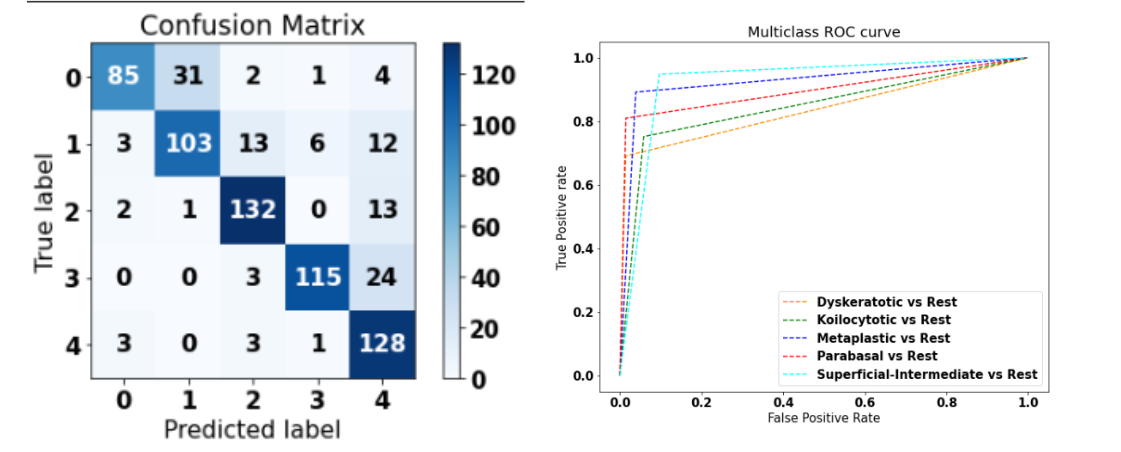
\includegraphics[width=160mm,height=55mm]{figures/cnn1.png}
\caption{Confusion Matrix and ROC\_AUC\_Curve with CNN 1 + Hyper-parameter Set 1}
\label{DLAccuracy}
\end{figure}

\begin{figure}[H]
\centering
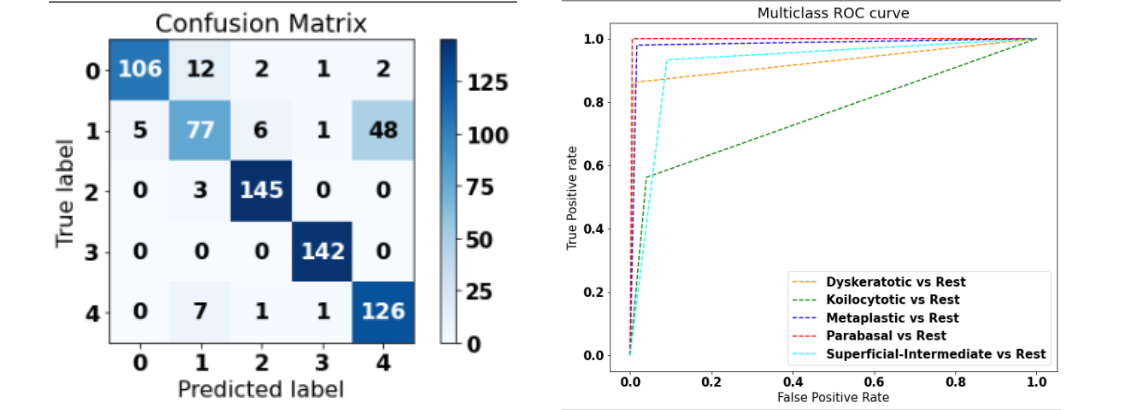
\includegraphics[width=160mm,height=55mm]{figures/cnn2.png}
\caption{Confusion Matrix and ROC\_AUC\_Curve with CNN 2 + Hyper-parameter Set 2}
\label{DLAccuracy}
\end{figure}

\begin{figure}[H]
\centering
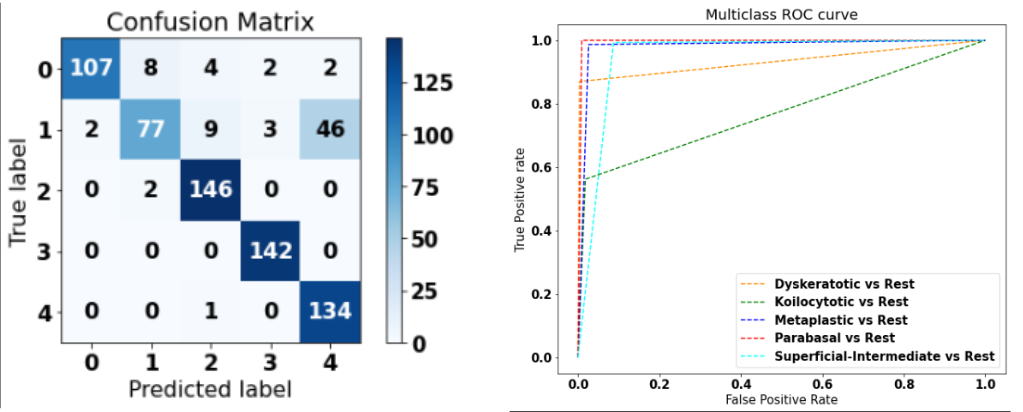
\includegraphics[width=160mm,height=60mm]{figures/cnn3.png}
\caption{Confusion Matrix and ROC\_AUC\_Curve with CNN 2 + Hyper-parameter Set 3}
\label{DLAccuracy}
\end{figure}

Figure-5.5, Figure-5.6, and Figure-5.7 show the confusion matrix on test data for the 3 configurations: CNN architecture 01+ Hyper-parameter Set 01,  CNN architecture 02+ Hyper-parameter Set 02, and  CNN architecture 02+ Hyper-parameter Set 03 respectively. The last configuration performs better as displayed by the One-Vs-Rest Multiclass ROC curve. Computing a ROC curve for each of the n classes constitutes the One-vs-the-Rest (OvR) multiclass technique, sometimes referred to as one-vs-all. A certain class is considered the positive class in each phase, and the remaining classes are collectively considered the negative class. It is evident from the plots that the AUC for each classes in the Configuration 3 ROC curve is higher than Configuration 1 and 2 ROC curves. Therefore, it can be said that CNN architecture 02 + Hyper-parameter set 03 did a better job of classifying amongst all configurations and also classical ML models. 


\pagebreak
\subsection{Prototype Development}
For deploying the proposed system in real-life environment a prototype was developed using streamlit and ngrok. There are two sides of the UI development: 
\begin{itemize}
    \item \textbf{Client Side} : In the client-side UI, a client can follow these necessary steps for training local model: enter the hospital/institution id, request for the global model parameters from the server, upload a zip file of training images, training the local model, send locally trained model parameters to the server and lasty test the global and local model with test images. 

    \begin{figure}[H]
    \centering
    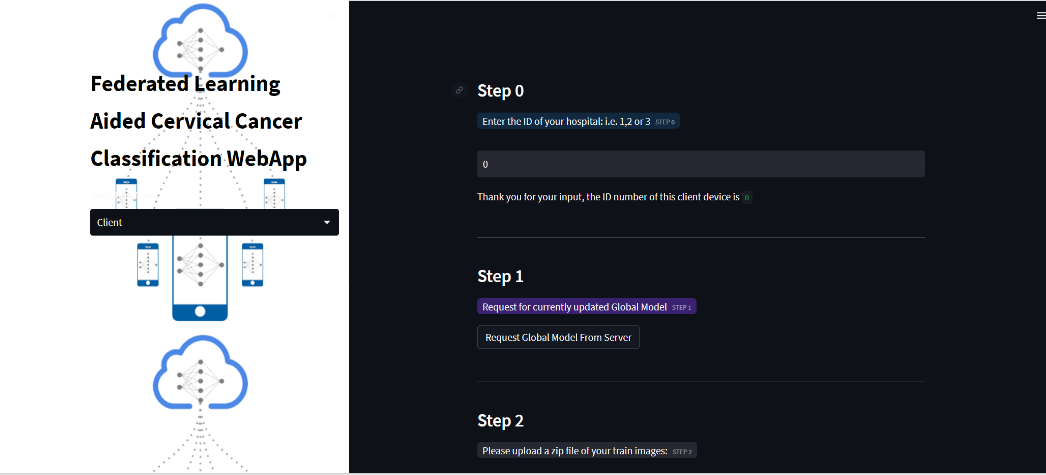
\includegraphics[width=160mm,height=70mm]{figures/frontend1.png}
    \caption{Development of Client-Side Frontend}
    \label{DLAccuracy}
    \end{figure}
    
    \begin{figure}[H]
    \centering
    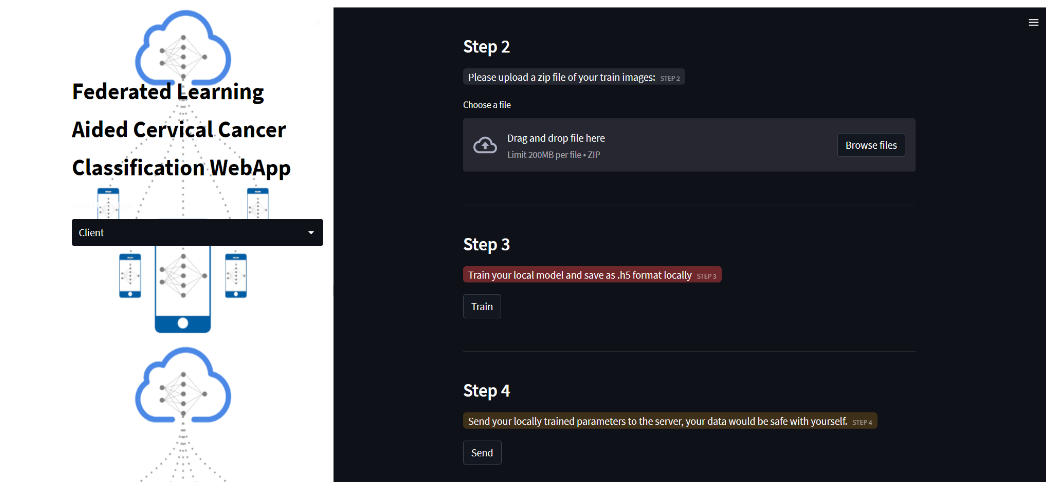
\includegraphics[width=160mm,height=70mm]{figures/frontend2.png}
    \caption{Development of Client-Side Frontend}
    \label{DLAccuracy}
    \end{figure}
    \item \textbf{Server Side} : In the server-side UI, an admin would first be authorized by entering a credential ID and then he can aggregate the local model updates with the global model.  
    
    \begin{figure}[H]
    \centering
    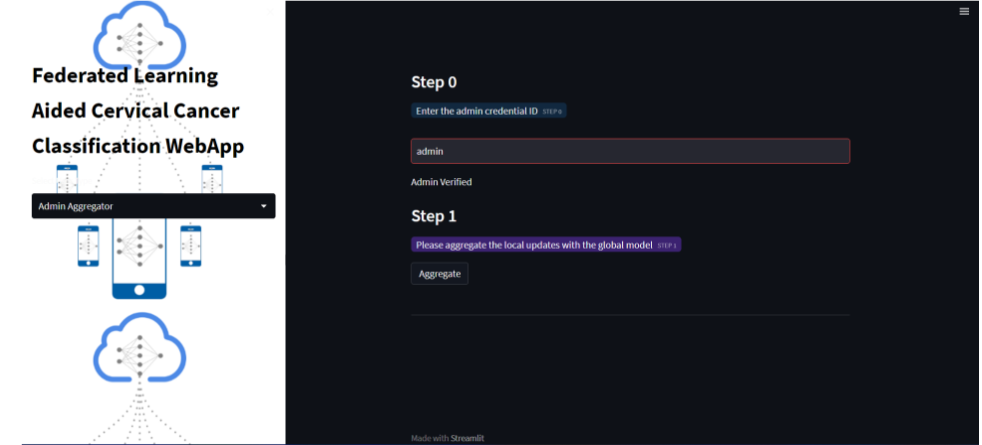
\includegraphics[width=160mm,height=70mm]{figures/frontend3.png}
    \caption{Development of Server-Side Frontend}
    \label{DLAccuracy}
    \end{figure}
\end{itemize}






% \begin{figure}[!h]
% \centering
% \includegraphics[width=6in]{figures/footPoseResnet50.pdf} %Texture
% \caption{\textcolor{black}{Development of Keypoint Estimation Model using ResNet50}}
% \label{fig:layers_of_model}
% \end{figure}

% \subsubsection{Layers utilized in the Model}
% \begin{itemize}
%     \item \textit{Conv2D(128, (3, 3), activation='relu', padding='same'):} This is a convolutional layer with 128 filters of size (3, 3) and a ReLU activation function. The padding='same' argument means that the output of the layer will have the same spatial dimensions as the input.
%     \item \textit{MaxPooling2D((2, 2)):}This is a max pooling layer that reduces the spatial dimensions of the output of the previous layer by a factor of 2. The layer takes the maximum value in each 2x2 window of the input.
%     \item \textit{Conv2D(64, (3, 3), activation='relu', padding='same'):} This is another convolutional layer with 64 filters of size (3, 3) and a ReLU activation function. The padding='same' argument means that the output of the layer will have the same spatial dimensions as the input.
%     \item \textit{MaxPooling2D((2, 2)):}  This is another max pooling layer that reduces the spatial dimensions of the output of the previous layer by a factor of 2.
%     \item \textit{Flatten():} This layer flattens the output of the previous layer into a 1D tensor, which can then be passed to a fully connected layer.
%     \item \textit{Dense(1024, activation='relu'):}  This is a fully connected layer with 1024 units and a ReLU activation function.
%     \item \textit{Dense(512, activation='relu'):} This is another fully connected layer with 512 units and a ReLU activation function.
%     \item \textit{Dense(8, activation='sigmoid'):} This is the final output layer with 8 units (one for each keypoint) and a sigmoid activation function. The linear activation function means that the output of the layer is not constrained to a particular range, so it can take any real value.
% \end{itemize}

% Thus the ML model was developed for keypoint estimation using the following parameters:
% % hyperparameters table
% \begin{table}[!ht]
% \caption{Hyperparameters used for Keypoint Estimation Model}
% \centering
% \begin{tabular}{p{6cm}p{6cm}}
% \hline
% \small \textbf{Parameters Used} & \small \textbf{Values}  \\
% \hline
% \small \textbf{Number of Conv2D layers} & \small 2 \\ 

% \small \textbf{Number of MaxPooling2D layers} & \small 2  \\

% \small \textbf{Number of Dense layers} & \small 3 \\

% \small \textbf{Number of units in the Dense layers} & \small 128, 512, and 8  \\

% \small \textbf{Activation functions used} & \small ReLU for Conv2D layers and Dense layers, and sigmoid for the output layer \\ 

% \small \textbf{Loss function} & \small Mean Squared Error (MSE) \\ 

% \small \textbf{Optimizer} & \small Adam \\ 

% \small \textbf{Input image size} & \small 224 x 224 x 3 (RGB image with 224 height, 224 width, and 3 channels) \\ 

% \small \textbf{BATCH_SIZE} & \small 32 \\ 

% \small \textbf{NUM_EPOCHS} & \small 100 \\ 

% \small \textbf{Learning Rate} & \small 0.001 \\ 
% \hline
% \end{tabular}
% \label{table:hyperparameters}
% \end{table}



